% SVN info for this file
\svnidlong
{$HeadURL$}
{$LastChangedDate$}
{$LastChangedRevision$}
{$LastChangedBy$}

\chapter{Connessione e compattezza}
\labelChapter{Connessocompatto}

\begin{introduction}
‘‘\emph{Lisa}: Allora, dov'è mio padre?\\
\emph{Professor Frink}: Beh, sarebbe ovvio anche per l'individuo più scriteriato, laureato e con specializzazione in Topologia iperbolica, che Homer Simpson è piombato... nella terza dimensione. [...] \emph{\textbf{[disegna sulla lavagna]}} Ecco un comunissimo quadrato—\\
\emph{Commissario Winchester}: Ehi ehi, rallenta, capuepopolo!\\
\emph{Professor Frink}: —ma supponiamo di estendere il quadrato oltre le due dimensioni del nostro universo, lungo l'ipotetica asse z, qui. \emph{\textbf{[tutti sussultano]}} Così si ottiene un oggetto tridimensionale noto come “cubo”, o meglio “Frinkaedro”, in onore dello scopritore!
\begin{flushright}
	\textsc{I Simpson,} La paura fa novanta VI.
\end{flushright}
\end{introduction}
\lettrine[findent=1pt, nindent=0pt]{L}{e} due proprietà che danno il nome a questo capitolo sono estremamente importanti, in quanto sono due dei principali \textit{invarianti} studiati in topologia. Entrambe rappresentano una \textit{generalizzazione} di alcuni aspetti affrontati più o meno esplicitamente durante lo studio dell'Analisi:
\begin{itemize}
	\item Ci sono sottoinsiemi del piano i cui punti possono essere \textit{connessi} da una linea arzigogolata, una spezzata o un segmento, mente
	\item Ci sono sottoinsiemi \textit{limitati} le cui successioni di punti \textit{convergono} nel sottoinsieme.
\end{itemize}
Vedremo che la \textbf{connessione} e la \textbf{compattezza} sono definite in modo abbastanza basilare, seppur non necessariamente siano intuitive a primo acchito. Tuttavia, proprio in virtù di questa semplicità, sono applicabili in tanti contesti diversi; in particolare, la compattezza come la definiremo ci permetterà di prendere informazioni note \textit{localmente} ed estenderle in modo che valgano globalmente in tutto lo spazio.
\section{Connessione}
\begin{define}[Spazio connesso e spazio sconnesso.]~{}\\
Uno spazio topologico $X$ si dice \textbf{connesso}\index{spazio!connesso} se gli unici sottoinsiemi aperti e chiusi sono $\emptyset,\ X$.\\
Uno spazio non \textit{connesso} si dice \textbf{sconnesso} oppure \textbf{non connesso}.
\end{define}
\begin{lemming}[Condizioni equivalenti della sconnessione; Manetti, 4.2.]~{}\label{sconnesso}\\
Sono condizioni equivalenti:
\begin{enumerate}
	\item $X$ è \textit{sconnesso}.
	\item $X=A\cup B$ con $A,\ B$ aperti, non vuoti, disgiunti.
	\item $X=A\cup B$ con $A,\ B$ chiusi, non vuoti, disgiunti.
\end{enumerate}
\vspace{-3mm}
\end{lemming}
\begin{demonstration}~{}\\
$2\iff3)$ Sono equivalenti: se $A$ è aperto e disgiunto da $B$ tale che $X=A\cup B$ significa che $B=\mathcal{C}A=X\setminus A$ e dunque chiuso; analogamente per $B$ aperto si ha che $A$ è chiuso: allora $A,\ B$ chiusi e aperti propri.\\
$1\implies2)$ Esiste $\emptyset\subsetneqq A \subsetneqq X$ con $A$ aperto e chiuso. Allora basta porre $B=\mathcal{C}A=X\setminus A$: essendo il complementare di $A$ è aperto e chiuso, sono disgiunti e tali per cui $B\neq X,\ B\neq \emptyset$. $A$ e $B$ soddisfano la tesi.\\
$1\implies2)$ $A$ aperto, $B$ aperto $\implies A$ chiuso perché $A=\mathcal{C}X=X\setminus B$. Inoltre $A$ non vuoto, $B$ non vuoto $\implies A\neq X$. Dunque $A$ è aperto, chiuso e $A\neq \emptyset,\ X$ e pertanto soddisfa la tesi: esiste un sottoinsieme aperto e chiuso che non il vuoto o l'insieme stesso.
\end{demonstration}
\begin{observe}
	Il lemma \ref{sconnesso} \textsc{(Manetti, 4.2)} ci dice che è sufficiente trovare solo due aperti (o chiusi) che soddisfano la condizione di cui sopra per affermare la sconnessione. Viceversa, per dimostrare la connessione, dobbiamo dimostrare che per ogni coppia di aperti (o chiusi) non vuoti, la cui unione è $X$, essi non siano disgiunti.
\end{observe}
\begin{examples} Esempi di spazi topologici \textit{sconnessi} in topologia Euclidea:
	\begin{itemize}
		\item $X=\realset\setminus\left\{0\right\}=\left(-\infty,\ 0\right)\cup \left(0,\ +\infty\right)$.
		\item $X=\left[0,\ 1\right]\cup \left(2,\ 3\right)$.
	\end{itemize}
\vspace{-3mm}
\end{examples}
\begin{lemming}[Un connesso è disgiunto o sottoinsieme di un aperto e chiuso; Manetti, 4.4.]~{}\\
Sia $X$ spazio topologico e $A\subseteq X$ con $A$ aperto e chiuso. Sia $Y\subseteq X,\ Y$ \textit{connesso}. Allora $Y\cap A=\emptyset$ (cioè $Y\subseteq Y\setminus A$) oppure $Y\subseteq A$.
\end{lemming}
\begin{demonstration}
Consideriamo $Y\cap A$: esso è intersezione di due aperti e chiusi per ipotesi ($Y$ è aperto e chiuso perché \textit{connesso}), cioè è aperto e chiuso. Essendo $Y$ \textit{connesso}, un suo sottoinsieme aperto e chiuso o è l'insieme vuoto oppure è l'insieme stesso, cioè $Y\cap A=\emptyset$ (cioè $Y\subseteq Y\setminus A$) oppure $Y\cap A=Y$ (cioè $Y\subseteq A)$.
\end{demonstration}
\begin{theorema}[Connessione di ${\left[0,\ 1\right]}$; Manetti, 4.6.]~{}\\
Con la topologia Euclidea, $X=\left[0,\ 1\right]$ è \textit{connesso}.
\end{theorema}
\begin{demonstration}
Supponiamo $X=\left[0,\ 1\right]=C\cup D$ con:
\begin{itemize}
	\item $C,\ D$ entrambi chiusi.
	\item $C,\ D$ entrambi aperti.
\end{itemize}
Dobbiamo dimostrare che $C,\ D$ \textit{non} sono disgiunti, ovvero $C\cap D\neq 0$. Supponiamo sia $0\in C$ e poniamo $d=\inf D$. Essendo $D$ un chiuso, $d\in \overline{D}=D$.
\begin{itemize}
	\item Se $d=0$, $d\in C\cap D\neq \emptyset$.
	\item Se $d>0$ allora $\left[0,\ d\right)\subseteq C$ perché \textit{non sta} in $D$. Il passaggio alla chiusura mantiene l'inclusione, dunque $\left[0,\ d\right]\subseteq \overline{C}=C$. Segue che $d\in C$ e dunque $C\cap D\neq \emptyset$.
\end{itemize}
\vspace{-3mm}
\end{demonstration}
\begin{theorema}[Immagine continua di un connesso è un connesso; Manetti, 4.7.]~{}\\
	L'immagine continua di un \textit{connesso} è un \textit{connesso}:
	\begin{equation}
		\funz{f}{X}{Y}\text{ continua},\ X\text{ connesso}\implies f\left(X\right)\text{ connesso}
	\end{equation}
\vspace{-6mm}
\end{theorema}
\begin{demonstration}
	Sia $Z\subseteq f\left(X\right)$, $Z$ aperto, chiuso in $f\left(X\right)$ non vuoto. Per dimostrare che $f\left(X\right)$ sia connesso ci è sufficiente dimostrare che $Z=f\left(X\right)$: in questo modo gli unici aperti e chiusi sono i sottoinsiemi impropri:
	\begin{itemize}
		\item $Z$ aperto: $\exists A$ aperto in $Y\ \colon Z=A\cap f\left(X\right)$.
		\item $Z$ chiuso: $\exists C$ chiuso in $Y\ \colon Z=C\cap f\left(X\right)$.
	\end{itemize}
Allora:
	\begin{itemize}
	\item $f^{-1}\left(Z\right)=f^{-1}\left(A\right)\cap f^{-1}\left(f\left(X\right)\right)=f^{-1}\left(A\right)\implies f^{-1}\left(Z\right)$ è uguale alla controimmagine continua di un aperto in $Y$, cioè è uguale ad un aperto di $X$.
	\item $f^{-1}\left(Z\right)=f^{-1}\left(C\right)\cap f^{-1}\left(f\left(X\right)\right)=f^{-1}\left(C\right)\implies f^{-1}\left(Z\right)$ è uguale alla controimmagine continua di un chiuso in $Y$, cioè è uguale ad un chiuso di $X$
	\end{itemize}
Segue che $f^{-1}\left(Z\right)$ è aperto e chiuso in $X$. Notiamo inoltre che, essendo $Z\neq \emptyset$, allora $f^{-1}\left(Z\right)\neq \emptyset$: essendo $X$ \textit{connesso} per ipotesi, necessariamente $f^{-1}\left(Z\right)=X$.
\end{demonstration}
\begin{observe}
Dal teorema precedente segue che essere \textit{connesso} è una proprietà topologica! Infatti, se vale per una qualunque funzione continua $\funz{f}{X}{Y}$, allora varrà anche per omeomorfismi tra $X$ e $Y$; in particolare, si avrà per suriettività che $f\left(X\right)=Y$ connesso.
\end{observe}
\subsection{Connessione per archi}
\begin{define}[Arco.]~{}\\
Un \textbf{arco}\seeonlyindex{arco}{cammino} o \textbf{cammino}\index{cammino} $\alpha$ da un punto $x$ a un punto $y$ in uno spazio topologico $X$ è una funzione continua che parametrizza un \textit{percorso} finito fra gli estremi $x$ e $y$:
\begin{equation}
\funz{\alpha}{\left[0,\ 1\right]}{X} \text{ continua}\ \colon \alpha\left(0\right)=x,\ \alpha\left(1\right)=y
\end{equation}
\vspace{-6mm}
\end{define}
\begin{define}[Connessione per archi.]~{}\\
Uno spazio topologico $X$ si dice \textbf{connesso per archi} o \textbf{c.p.a.}\index{spazio!connesso per archi}\seeonlyindex{spazio!c.p.a.}{spazio!connesso per archi} o \textit{path-connected} se per ogni coppia di punti in $X$ esiste un arco che li collega:
\begin{equation}
\forall x,\ y\in X\ \exists \funz{\alpha}{\left[0,\ 1\right]}{X} \text{ continua}\ \colon \alpha\left(0\right)=x,\ \alpha\left(1\right)=y
\end{equation}
\vspace{-6mm}
\end{define}
\begin{theorema}[$X$ c.p.a. implica $X$ connesso; Manetti, 4.7.]~{}\\
\end{theorema}
\begin{demonstration}
	Sia $X=A\cup B$, con $A,\ B$ aperti non vuoti. Vogliamo dimostrare che $A\cap B\neq \emptyset$. Essendo non vuoti, prendiamo $a\in A,\ b\in B$. In quanto $X$ è \textbf{c.p.a.}, esiste il cammino (continuo) $\funz{\alpha}{\left[0,\ 1\right]}{X}$ tale che $\alpha\left(a\right)=a,\ \alpha\left(1\right)=b$.\\
	Studiamo la controimmagine di $\alpha$:
	\begin{gather*}
		\alpha^{-1}\left(X\right)=\alpha^{-1}\left(A\cup B\right)=\left[0,\ 1\right]\\
		\left[0,\ 1\right]=\alpha^{-1}\left(A\cup B\right)=\alpha^{-1}\left(A\right)\cup \alpha^{-1}\left(B\right)
	\end{gather*}
$\alpha^{-1}\left(A\right),\ \alpha^{-1}\left(B\right)$ sono entrambi aperti e non vuoti in quanto controimmagini (continue) di aperti non vuoti ($0\in \alpha^{-1}\left(A\right),\ 1\in \alpha^{-1}\left(B\right)$).\\
Poiché $\left[0,\ 1\right]$ è connesso, allora le controimmagini trovate non sono disgiunte. Segue allora:
\begin{equation*}
\exists t\in \alpha^{-1}\left(A\right)\cap \alpha^{-1}\left(B\right)\implies \alpha\left(t\right)\alpha\left(\alpha^{-1}\left(A\right)\cap \alpha^{-1}\left(B\right)\right)\subset\alpha\left(\alpha^{-1}\left(A\right)\right)\cap\alpha\left(\alpha^{-1}\left(B\right)\right)=A\cap B
\end{equation*}
\end{demonstration}
\begin{define}[Giunzione di cammini.]~{}\\
	Dati due cammini in uno spazio $X$:
	\begin{gather*}
		\funz{\alpha}{\left[0,\ 1\right]}{X}\quad \alpha\left(0\right)=x,\ \alpha\left(1\right)=y\\
		\funz{\beta}{\left[0,\ 1\right]}{X}\quad \beta\left(0\right)=y,\ \beta\left(1\right)=z
	\end{gather*}
	Allora possiamo creare un cammino $\alpha \ast \beta$ con la \textbf{giunzione di cammini}\index{cammino!giunzione di cammini}:
	\begin{equation}
		\left(\alpha\ast\beta\right)\left(t\right)=\begin{cases}
			\alpha\left(2t\right)\quad\text{se }0\leq t\leq \frac{1}{2}\\
			\beta\left(2t-1\right)\quad\text{se }\frac{1}{2}\leq t\leq 1\\	
		\end{cases}
	\end{equation}
\vspace{-6mm}
\end{define}
\begin{lemming}[Unione di c.p.a. non disgiunta è c.p.a.]~{}\\
	Sia $A,\ B$ \textbf{c.p.a}, $A\cap B\neq \emptyset\implies A\cup B$ \textbf{c.p.a.}
\end{lemming}
\begin{demonstration}
	Se $x, y\in A$ oppure $x,\ y\in B$ esiste per ipotesi un arco che li collega. Dobbiamo allora trovare un arco in $A\cup B$ da $x$ a $y$ $\forall x\in A, y\in B$. Preso $z\in A\cap B$, per ipotesi esistono due cammini ad esso:
	\begin{gather*}
		\funz{\alpha}{\left[0,\ 1\right]}{A}\quad \alpha\left(0\right)=x,\ \alpha\left(1\right)=z\\
		\funz{\beta}{\left[0,\ 1\right]}{B}\quad \beta\left(0\right)=z,\ \beta\left(1\right)=z	
	\end{gather*}
	Usando la \textit{giunzione di cammini}, si ha:
	\begin{equation}
		\left(\alpha\ast\beta\right)\left(t\right)=\begin{cases}
			\alpha\left(2t\right)\quad\text{se }0\leq t\leq \frac{1}{2}\\
			\beta\left(2t-1\right)\quad\text{se }\frac{1}{2}\leq t\leq 1\\	
		\end{cases}
	\end{equation}
	Il cammino $\funz{\alpha\ast\beta}{\left[0,\ 1\right]}{A\cup B}$ è quello richiesto.
\end{demonstration}
\begin{observes}~{}\label{giunzionecpa}
	\begin{itemize}
		\item Usando la giunzione di cammini, si ha che:
		\begin{equation*}
			X\text{ è \textbf{c.p.a.}}\iff \exists z\in X\ \colon \forall x\in X\quad
			\exists \funz{\alpha}{\left[0,\ 1\right]}{X}\ \colon \alpha\left(0\right)=z,\ \alpha\left(1\right)=x
		\end{equation*}
		In altre parole, uno spazio è \textbf{c.p.a.} se e solo se esiste un punto per cui ogni altro punto è collegato tramite un arco.
		\item Per ogni arco $\alpha$ esiste l'arco inverso, percorso al contrario: $\overline{\alpha}\left(t\right)=\alpha\left(1-t\right)$.
	\end{itemize}
\vspace{-3mm}
\end{observes}
\begin{define}[Segmento.]~{}\label{segmento}\\
In $\realset^n$, un \textbf{segmento}\index{segmento} $\overline{PQ}$ è la combinazione lineare tra i punti $P$ e $Q$, parametrizzato come:
	\begin{equation}
		\overline{PQ}=\left\{P+tQ\mid t\in\left[0,\ 1\right]\right\}
	\end{equation}
\vspace{-6mm}
\end{define}
\begin{define}[Sottoinsieme convesso.]~{}\\
	Un sottoinsieme $Y\subseteq\realset^n$ è \textbf{convesso}\index{sottoinsieme!convesso} se per ogni coppia di punti esiste un segmento che li collega contenuto interamente in $Y$.
	\begin{equation}
		\forall P,\ Q\in Y\quad \overline{PQ}\subseteq Y
	\end{equation}
\vspace{-6mm}
\end{define}
\begin{define}[Sottoinsieme stellato.]~{}\\
	Un sottoinsieme $Y\subseteq\realset^n$ è \textbf{stellato}\index{sottoinsieme!stellato} per $P$ se esiste un $P\in Y$ tale che per ogni altro punto esiste un segmento che li collega contenuto interamente in $Y$.
	\begin{equation}
		\exists P \in Y\ \colon \forall Q\in Y\quad \overline{PQ}\subseteq Y
	\end{equation}
\vspace{-6mm}
\end{define}
\begin{examples}~{}
\begin{itemize}
	\item Gli intervalli aperti e semiaperti sono \textbf{c.p.a}, dunque sono \textit{connessi}: l'arco $\alpha$ è banalmente il segmento pari all'intervallo aperto.
	\item Preso $X\subseteq\realset^n$ \textit{convesso}, qualunque segmento è anche per costruzione un arco: $X$ è anche \textbf{c.p.a} e dunque \textit{connesso}.
	\item $X=\realset^{2}\setminus\left\{0\right\}$ \textit{non} è \textit{convesso} (per $\left(0,\ 1\right)$ e $\left(0,\ -1\right)$ non si hanno segmenti interni ad $X$) ma è \textbf{c.p.a.} (basta prendere un cammino che ‘‘giri attorno'' all'origine) e dunque è \textit{connesso}.
	\item Preso $X\subseteq\realset^n$ \textit{stellato} per $P\in X$, qualunque segmento con $P$ è anche per costruzione un arco: $X$ è anche \textbf{c.p.a} per l'osservazione \ref{giunzionecpa} e dunque {connesso}.
	\item Ogni insieme \textit{convesso} è anche \textit{stellato} per $P$, basta fissare un qualunque punto come nostro $P$. In generale, un insieme è convesso se e solo se è stellato per ogni suo punto.
\end{itemize}
\vspace{-3mm}
\end{examples}
\subsection{Connessione nella topologia euclidea}
Vediamo ora che conseguenze hanno questi teoremi in $\realset$ con la topologia Euclidea.
\begin{theorema}[Condizioni equivalenti della connessione su $\realset$.]~{}\\
	Sia $I\subseteq \realset$. Le seguenti affermazioni sono equivalenti:
		\begin{enumerate}
	\item $I$ è un intervallo, ovvero $I$ è \textit{convesso}.
	\item $I$ è \textbf{c.p.a.}.
	\item $I$ è connesso.
		\end{enumerate}
	\vspace{-3mm}
\end{theorema}
\begin{demonstration}~{}\\
	$1) \implies 2)$ Siccome $I$ è convesso $\implies$ $I$ stellato $\implies$ $I$ \textbf{c.p.a.} $\implies$ $I$ connesso. \\
	$2) \implies 3)$ Vale in generale che \textbf{c.p.a.} $\implies$ connesso.\\
	$3) \implies 1)$ Per contronominale mostriamo che $I$ non intervallo $\implies$ $I$ sconnesso. $I$ non intervallo significa che
		\begin{gather*}
			\exists a<b<c,\ a,c\in I,\ b\notin I \\
			b\notin I \implies I= \left(\underbrace{ I\cap \left(-\infty ,b\right)}_{\in a}\ \right) \cup \left( \underbrace{I\cap \left(b ,+\infty\right)}_{\in c}\ \right)
		\end{gather*}
	ovvero $I$ è unione di aperti, non vuoti e disgiunti $\implies$ $I$ sconnesso.	
\end{demonstration}
\begin{observe}~{}\label{teorema esistenza zeri funzioni continue, s^n cpa}
		\begin{itemize}
	\item Come conseguenza immediata di questo teorema si ha il \textbf{teorema di esistenza degli zeri}\index{teorema! di esistenza degli zeri} per funzioni continue da $\realset$ in $\realset$, infatti se l'immagine continua di un connesso è un connesso, per tali funzioni vale che l'immagine continua di un intervallo è un intervallo.
	\item Per $n\geq 1$ la \textbf{sfera}\index{sfera} $\displaystyle S^n \coloneqq \left\{ \left(x_1,\dots,x_{n+1}\right) \mid \sum_{i=1}^{n+1}x_i^2=1 \right\}$ è \textbf{c.p.a.}; infatti, $\forall x,y\in S^n$ si trova sempre un arco dato dall'intersezione di $S^n$ e del piano $H$ passante per il centro della sfera, $x$ e $y$.
		\end{itemize}
	\vspace{-3mm}
\end{observe}
Mostriamo un risultato per funzioni continue da $S^n$ in $\realset$.
\begin{theorema}[Funzioni continue da continue da $S^n$ in $\realset$.]~{}\label{non iniettività S^n in realset}\\
Sia $\funz f {S^n} \realset$ una funzione continua. Allora $\exists x\in S^n \ \colon f(x)=f(-x)$. In particolare $f$ non è iniettiva.
\end{theorema}
\begin{demonstration}
	Costruiamo una funzione $g(x)=f(x)-f(-x)$: essa è continua perché somma di funzioni continue. Siccome $S^n$ è connesso allora $g\left( S^n\right)\subseteq\realset$ è connesso $\implies$ per il teorema precedente $g\left(S^n\right)$ è un intervallo.\\
	Si considerino un punto $y\in S^n$ arbitrario e le sue immagini $g(y)$ e $g(-y)$: esse appartengono all'intervallo dell'immagine $g\left( S^n\right)$, quindi se ne può considerare il loro punto medio:
		\begin{gather*}
			\frac{1}{2}\left[ g(y) - g(-y)\right]=\frac{1}{2} \left[ f(y) -f(-y) - f(y) +f(-y) \right]= 0\\
			\implies \exists x\in S^n \colon g(x)=0, \text{ ovvero } f(x)=f(-x)
		\end{gather*}
\end{demonstration}
Come conseguenza di questo teorema si ha che un aperto di $\realset$ non sarà mai omeomorfo ad un aperto di $\realset^n$.
\begin{theorema}[Aperti di $\realset$ non omeomorfi ad aperti di $\realset^n$.]~{}\\
Sia $I\subseteq\realset$ e $U\subseteq\realset^n$, con $n\geq 2$. Se $I,\ U$ sono aperti allora $I$ non è omeomorfo a $U$.	
\end{theorema}	
\begin{demonstration}
	Si consideri un omeomorfismo $\funz g U I$. Siccome $U\subseteq\realset^n$ aperto allora esiste una palla aperta di raggio $\epsilon$ contenuta in $U$, se ne considera il bordo $S^n\subseteq U$. Si considera dunque la restrizione $\funz {g_{|_{S^n}}} {S^n} I$, che per il teorema precedente non è iniettiva. Dunque $g$ non è un omeomorfismo.	
\end{demonstration}

\begin{observe}
	Il teorema appena visto è un caso particolare del \textsc{teorema dell'invarianza della dimensione}\index{teorema!dell'invarianza della dimensione}: ‘‘Siano $U\subseteq\realset^n, V\subseteq\realset^m$ aperti. Se $U\cong V \implies n=m$. Equivalentemente $n\neq m\implies U\ncong V$''.
\end{observe}
% LEZ 08
\subsection{Intersezioni, unioni e prodotti di spazi connessi}
\begin{theorema}[Unione arbitraria di sottospazi connessi è un connesso.]~{}\label{unione sottospazi connessi}\\
Siano $\left\{ X_i \right\}_{i\in I}$ una famiglia di sottoinsiemi di uno spazio topologico $X$. Se ogni $X_i$ è connesso e $\displaystyle\inter_{i\in I}X_i\neq\emptyset$ allora $\displaystyle\union_{i\in I}X_i$ è connesso.	
\end{theorema}
\begin{demonstration}
	Sia $\displaystyle Z\subseteq Y\coloneqq \union_{i\in I}X_i$ un aperto, chiuso non vuoto. Vogliamo dimostrare che $Z=X$, cosicché $X$ risulti connesso. Basta l'inclusione $Y\subseteq Z$.\newline
	Si considera l'intersezione di $Z$ e di un connesso, dunque essa sarà banale:
	\begin{gather*}
		X_i \cap Z = \begin{cases}
			\emptyset & \\
			X_i	&		
		\end{cases}
	\end{gather*}
	Dimostriamo ora che non è vuota, infatti siccome $Z$ non è vuoto ed è contenuto nell'unione ci sarà un connesso per cui l'intersezione non è vuota:
		\begin{gather*}
			Z\neq\emptyset, \ Z\subseteq \union_{i\in I}X_i \implies \exists i_0 \ \colon X_{i_0}\cap Z\neq \emptyset	\\
			X_{i_0} \text{ è connesso } \implies X_{i_0}\cap Z=X_{i_0} \implies X_{i_0}\subseteq Z \\
			\text{Siccome } \inter_{i\in I}X_i\neq\emptyset \implies \exists x\in\inter_{i\in I}X_i \implies x\in X_{i_0}\subseteq Z \implies x\in Z	\\
			\text{Siccome } x\in\inter_{i\in I}X_i \text{e} x\in Z \implies \forall i\in I, \ X_i\cap Z\neq\emptyset
		\end{gather*}
	Quindi per $\forall i, \ X_i\subseteq Z \implies Y\subseteq Z \implies Y=Z$, quindi $Y$ è connesso perché l'unico aperto e chiuso non vuoto è banale ($Y$).
\end{demonstration}

\begin{theorema}[Prodotto di connessi è connesso.]~{}\label{prodotto connessi}\\
$X, Y$ sono spazi topologici connessi $\iff X\times Y$ è connesso.	
\end{theorema}
\begin{demonstration}~{}\\
	$\impliessx$ Si sfrutta la continuità delle proiezioni e che l'immagine continua di un connesos è connessa:
		\begin{gather*}
			\funz p {X\times Y} X \text{continua e suriettiva } \implies p(X)=X \text{ connesso}\\
			\funz q {X\times Y} Y \text{continua e suriettiva } \implies q(Y)=Y \text{ connesso}	
		\end{gather*}	
	$\impliesdx$ Si vuole sfruttare il teorema sull'unione di connessi, prestando attenzione che la loro intersezione non sia vuota, quindi si scrive il prodotto come unione di connessi già noti:
	$\displaystyle X\times Y=\union_{y\in Y}X\times\{y\}$, infatti $X\times\{y\}\cong X$ che per ipotesi è connesso , tuttavia $\displaystyle\inter_{y\in Y}X\times\{y\}=\emptyset$ !\newline
	Cerchiamo dunque di unire un insieme in modo tale che l'intersezione non sia vuota: sia $x_0\in X$ e $Y_{x_0}=\{x_0\}\times Y$ e poniamo $X_y=X\times\{y\}$ e si ha quanto voluto:
		\begin{gather*}
			X\times Y=\union_{y\in Y}X_y \cup Y_{x_0} \text{ e } X_y\cap Y_{x_0}=(x_0,y)\\
			\implies \inter_{y\in Y}\left( X_y  \cup Y_{x_0}\right)\neq\emptyset		
		\end{gather*}
	Dunque $X\times Y$ è unione di connessi la cui intersezione non è vuota, quindi per il teorema precedente è connesso.
\end{demonstration}
\subsection{Spazi connessi non c.p.a.}
Approfondiamo ora la differenza fra essere spazio connesso o \textbf{c.p.a.}, mostrando esempi di un tipo ma non dell'altro. Prima, però, dimostreremo un teorema sulla caratterizzazione di un \textit{insieme denso} che ci tornerà utile.
\begin{theorema}[Caratterizzazione di un insieme denso.]~{}\\
	Sia $X$ uno spazio topologico e $A\subseteq X$ un suo sottoinsieme, allora:
		\begin{gather*}
			A \text{ è denso }\iff \forall U\subseteq X \text{ aperto e } \ U\neq\emptyset, \ \ U\cap A\neq\emptyset	
		\end{gather*}
	\vspace{-6mm}
\end{theorema}
\begin{demonstration}~{}
	$\impliesdx$ Se $A$ è denso allora $\overline{A}=X$. Supponiamo che $\exists V$ aperto $\colon V\cap A=\emptyset$. Siccome $V$ è aperto allora $X\setminus V$ è chiuso, inoltre $V\cap A=\emptyset$, quindi $A\subseteq X\setminus V$. Essendo $A$ contenuto in un chiuso allora lo sarà anche la sua chiusura, siccome è il più piccolo chiuso che lo contiene:
		\begin{gather*}
			\overline{A}=X\subseteq X\setminus V \implies V=\emptyset
		\end{gather*}
	Ne segue che l'unico aperto che non interseca $A$ è l'insieme vuoto. \newline
	$\impliessx$ Consideriamo un chiuso $K\supseteq A$. Siccome è chiuso allora il suo complementare $X\setminus K$ è aperto. Per ipotesi dunque si ha che $V\cap A\neq \emptyset$ oppure $V=\emptyset$, passando al complementare si ottiene che:
		\begin{equation*}
			\begin{array}{l}
				A\subseteq K \implies X\setminus K \subseteq X\setminus A \implies V\subseteq X\setminus A \implies \\
				\implies V\cap A=\emptyset \implies V=\emptyset \implies K=X \implies \overline{A}=X
			\end{array}
		\end{equation*}
	L'ultima implicazione è dovuta al fatto che ogni chiuso che contiene $A$ si è dimostrato essere solo $X$ per cui esso sarà la sua chiusura.
\end{demonstration}

\begin{theorema}[Chiusura e connessione.]~{}\label{chiusuraconnessa}\\
Sia $X$ uno spazio topologico e $Y\subseteq X$ connesso, allora
		\begin{equation*}
			\forall W \colon Y\subseteq W \subseteq \overline{Y} \implies W \text{ connesso}
		\end{equation*}
	In particolare la chiusura di un connesso è connessa.
\end{theorema}
\begin{demonstration}
	Per dimostrare che $W$ è connesso si considera un suo sottoinsieme $Z\subseteq W$ aperto, chiuso e non vuoto e si mostra che è pari a $W$.
		\begin{gather*}
			Z\subseteq W \text{ aperto } \implies \exists A\subseteq X \text{ aperto } \colon Z=W\cap A \\
			Z\subseteq W \text{ chiuso } \implies \exists C\subseteq X \text{ chiuso } \colon Z=W\cap C
		\end{gather*}
	Si vuole sfruttare il fatto che $Y$ è connesso:
		\begin{gather*}
			Z\cap Y=A\cap W\cap Y \stackrel{!}{=} A\cap Y \text{ aperto in Y}
			Z\cap Y=C\cap W\cap Y \stackrel{!}{=} C\cap Y \text{ aperto in Y}			
		\end{gather*}
	Dove il passaggio indicato con (!) è dovuto al fatto che $Y\subseteq W$. Per poter sfruttare la connessione di $Y$ e dedurre che $Z\cap Y=Y$ dobbiamo prima provare che tale intersezione non è vuota e per farlo sfruttiamo il teorema precedente:
		\begin{gather*}
			Y \text{ denso in W, infatti  } \mathcal{cl}_W(Y)=\mathcal{cl}_X(Y)\cap W=\overline{Y}\cap W=W\\
			Z \text{ aperto in } W \implies Z\cap Y \neq \emptyset \implies Z\cap Y=Y \implies Y\subseteq Z
		\end{gather*}
	Tuttavia $Y$ è denso in $W$ e $Z$ è chiuso in $W$ che contiene $Y$, quindi
		\begin{equation*}
			\mathcal{cl}_W(Y)=W\subseteq Z \implies W=Z \implies W \text{ connesso}
		\end{equation*}
\end{demonstration}
Vediamo ora degli esempi di spazi connessi ma non \textbf{c.p.a.}.
\begin{example}\textsc{Seno del topologo.}\\
\begin{minipage}{0.47\textwidth}
Sia $Y\subseteq \realset^2$ con la topologia euclidea e $Y=\left\{ \left( x,\ \frac{1}{x} \right) \mid x>0 \right\}$, detto anche \textbf{seno del topologo}\index{seno del topologo}. Esso è \textbf{c.p.a.} perché per connettere due punti basta percorrere la curva stessa del grafico. Quindi $Y$ è connesso, dunque per il teorema \ref{chiusuraconnessa} (pag. \pageref{chiusuraconnessa}) $\overline{Y}$ è connesso.\\
Tuttavia $\overline{Y}$ non è \textbf{c.p.a.} in quanto $\overline{Y}=Y\cup \left\{ (0,y) \mid -1\leq y \leq 1 \right\}$ ed i punti sull'asse delle $y$ e sulla curva $Y$ non si possono connettere tramite un arco continuo.
\end{minipage}
\hspace{-7mm}
\begin{minipage}{0.52\textwidth}
	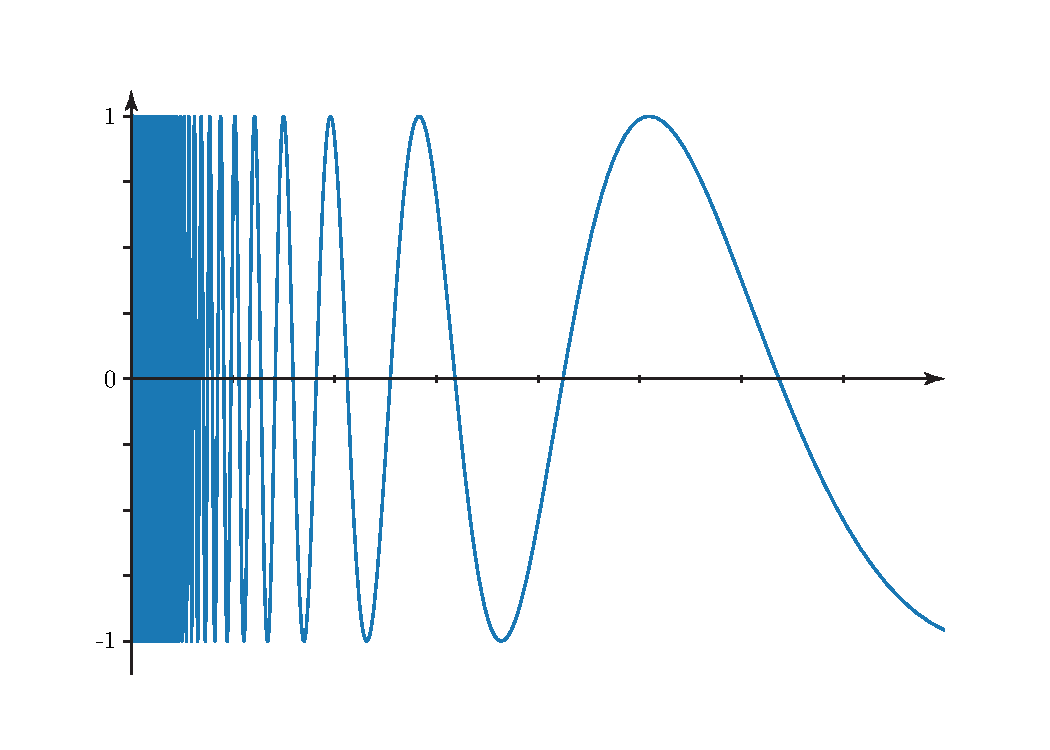
\includegraphics[trim=0cm 0.5cm 0.5cm 1.25cm,clip,scale=0.50]{images/topologistsine.pdf}
\end{minipage}
\end{example}
\begin{example}\textsc{La pulce ed il pettine.}\\
	Si consideri il ‘‘pettine'' come il seguente sottospazio di $\realset ^2$ con la topologia euclidea:
		\begin{equation*}
			Y= \left\{ (x,\ 0) \mid 0\leq x\leq 1 \right\} \cup \union_{\stackrel{r\in\rationalset}{ 0\leq r\geq 1}} \left\{ (r,\ y) \mid 0\leq y \leq 1 \right\}
		\end{equation*}
\begin{minipage}{0.62\textwidth}
Presi due punti su $Y$ si possono collegare fra loro scendendo alla base del pettine $\left[0,\ 1\right]$ e risalendo sui ‘‘denti'' di ascissa razionale. Quindi $Y$ è \textbf{c.p.a.}, allora $Y$ è connesso e $\overline{Y}=\left[0,\ 1\right]\times \left[0,\ 1\right]$.\newline
Si consideri ora la ‘‘pulce'', ovvero un punto $P$ di ascissa irrazionale ed ordinata 1, ad esempio $P=\left(\frac{\sqrt{2}}{2},\ 1\right)$. Sia $Z=Y\cup P$; per il teorema precedente segue che $Z$ è connesso, infatti:
\begin{gather*}
	Y\subseteq Z \subseteq \overline{Y}=\left[0,\ 1\right]\times \left[0,\ 1\right]	
\end{gather*}
	\end{minipage}
	\begin{minipage}{0.37\textwidth}
		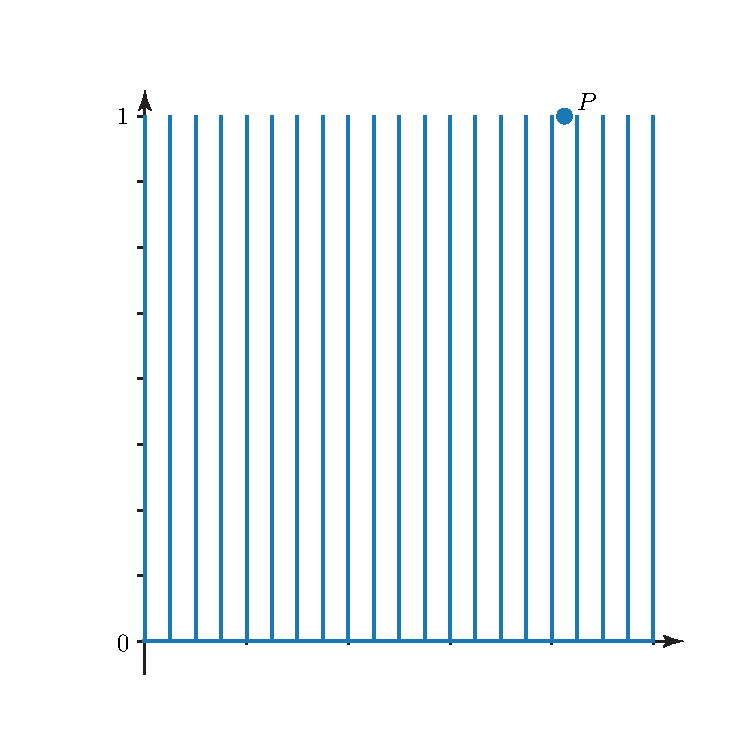
\includegraphics[trim=1.1cm 0.5cm 0.5cm 1.25cm,clip,scale=0.50]{images/comb.pdf}
	\end{minipage}\\
Tuttavia $Z$ non è \textbf{c.p.a.}: preso un cammino $\funz \alpha {\left[0,\ 1\right]} {Z\subseteq \realset^2}$ tale che $\alpha(t)= \left( x(t), y(t)\right)$ con $\alpha (0)=(0,0)$ e $\alpha(1)=P$, per continuità $y(t)\neq 0 \implies x(t)\in\rationalset$, ma è vero per $P$ che ha ascissa irrazionale, dunque non esiste un cammino continuo che colleghi l'origine e $P$. Ne consegue che $Z$ non è \textbf{c.p.a.}.
\end{example}

\begin{observe}
	L'immagine continua di uno spazio \textbf{c.p.a.} è \textbf{c.p.a.}, ovvero dato $X$ \textbf{c.p.a.}, $\funz f X Y$ continua, allora $f(X)$ è \textbf{c.p.a.}.\newline
	Dati $a,b\in X$ si vuole trovare un cammino fra $f(a)$ e $f(b)$ in $f(X)$. Si consideri la composizione seguente fra il cammino $\alpha$ fra $a$ e $b$ con la funzione $f$ stessa. Siccome ha come dominio $\left[0,\ 1\right]$ ed è continua essendo composizione di funzione continue è in effetti un cammino fra le due immagini:
\begin{center}
\begin{tikzcd}
	{f\circ \alpha\ \colon \left[0,\ 1\right]} \arrow[r, "\alpha"] & X \arrow[r, "f"] & Y
\end{tikzcd}
\end{center}
\vspace{-6mm}
\end{observe}
\subsection{Componenti connesse}
L'intuizione geometrica che ci ha portati alla definizione di connessione è stata ‘‘di quanti pezzi è fatto uno spazio?''. Se uno spazio è connesso è fatto di un solo ‘‘pezzo'', cerchiamo ora di definire cosa sono i ‘‘pezzi'' e come sono fatti.
\begin{define}[Componente connessa.]~{}\\
	Sia $X$ uno spazio topologico e $C\subseteq X$. Si dice che $C$ è una \textbf{componente connessa}\index{componente!connessa} se:
		\begin{itemize}
			\item $C$ è \textit{connesso}.
			\item $C$ è \textbf{massimale}\index{massimale}, ovvero $C\subseteq A$, $A$ connesso $\implies C=A$.
		\end{itemize}
	Scelto $x\in X$ si può definire la \textbf{componente connessa di un punto}\index{componente!connessa di un punto}, ovvero:
	\begin{equation}
		\displaystyle C(x)=\union \{C \mid C\text{ connesso},\ x\in C\}
	\end{equation}
\vspace{-6mm}
\end{define}
La componente connessa di \textit{un punto} è effettivamente una componente connessa: infatti, è connessa perché unione di connessi con intersezione \textit{non vuota} ($x$ stesso) e se $C(x)\subseteq A \implies x\in A \implies A\subseteq C(x) \implies A=C(x)$.\newline
Vediamo ora qualche proprietà delle componenti connesse, in particolare che sono chiuse e formano una partizione.
\begin{theorema}[Componenti connesse sono chiuse e partizione.]~{}\\
	Sia $X$ uno spazio topologico, allora:
		\begin{enumerate}
			\item le componenti connesse sono chiuse.
			\item le componenti connesse formano una partizione di $X$.
		\end{enumerate}
	\vspace{-3mm}
\end{theorema}
\begin{demonstration}
	~{}
	\begin{enumerate}[label=\Roman*]
		\item Sia $C$ una componente connessa. Per ogni insieme vale che $C\subseteq\overline{C}$, ma $C$ è connesso, quindi $\overline{C}$ è connesso. Siccome $C$ è massimale allora $C=\overline{C}$, ovvero è chiuso.
		\item Per dimostrare che le componenti connesse formano una partizione di $X$ dobbiamo mostrare che $X$ è unione disgiunta delle componenti connesse. Prima di tutto dimostriamo che sono un ricoprimento
			\begin{equation*}
				\forall x\in X,\ x\in C(x) \implies X=\union_{x\in X}C(x)
			\end{equation*}
		Mostriamo ora che sono disgiunti prendendo due componenti connesse $C$ e $D$ ed analizzando il caso in cui la loro intersezione non è vuota, in particolare sfruttiamo la massimalità:
		\begin{gather*}
			C\cap D\neq\emptyset \implies C\cup D \text{ connesso } \implies C=C\cup D=D
		\end{gather*}
	\end{enumerate}
\vspace{-6mm}
\end{demonstration}
\begin{example}
	Sia $\rationalset\subseteq\realset$ con la topologia Euclidea. La componenti connesse di $\rationalset$ sono i punti, quindi i punti sono chiusi in $\rationalset$, il che è una riconferma dato che sappiamo che $\rationalset$ è Hausdorff. Tuttavia non possono essere aperti altrimenti avremmo la topologia discreta!\newline
	Inoltre siccome $\rationalset$ ha più di una componente connessa significa che non è connesso! Invece $\realset$ è connesso grazie all'assioma di completezza.
\end{example}
\begin{observe}
	Dati due spazi omeomorfi si ha che hanno lo stesso numero di componenti connesse in quanto l'immagine continua di connessi è connessa. Quindi il \textbf{numero di componenti connesse} ci fornisce un criterio per determinare quando due spazi non sono omeomorfi!
\end{observe}


		\section{Compattezza}
\begin{define}[Ricoprimento aperto e sottoricoprimento.]~{}\\
	Sia $X$ uno spazio topologico. Un \textbf{ricoprimento aperto}\index{ricoprimento}\index{ricoprimento!aperto} di $X$ è una famiglia $\mathcal{A}=\{A_i \}_{i\in I}$ di aperti di $X$ tali che $X=\union_{i\in I} A_i$. \newline
	Un \textbf{sottoricoprimento}\index{sottoricoprimento} $\mathcal{B}$ di un ricoprimento aperto $\mathcal{A}$ è una famiglia di aperti di $\mathcal{A}$ la cui unione è ancora tutto $X$.
\end{define}		

\begin{examples}\textsc{Esempi di ricoprimenti aperti.}
	\begin{itemize}
		\item $\displaystyle \realset=(-\infty ,\ 2)\cup(0,\ +\infty)$ è un ricoprimento aperto
		\item $\displaystyle \realset =\union_{n\in\naturalset}(n,\ -n)$ è un ricoprimento aperto
		\item $\displaystyle \realset=\union_{p \text{ primo}}(-p,p)$ è un ricoprimento aperto
	\end{itemize}
\end{examples}

\begin{define}[Spazio compatto.]~{}\\
	Uno spazio topologico $X$ si dice \textbf{compatto}\index{spazio!compatto} se dato un qualsiasi ricoprimento aperto $\mathcal{A}$ si può sempre estrarre un sottoricoprimento \textit{finito} $\mathcal{B}$.
\end{define}
L'importanza della definizione risiede nel fatto che non si chiede che esista un ricoprimento $\mathcal{A}$ finito (basterebbe banalmente $X$ stesso che è aperto) bensì che da $\mathcal{A}$ si possa sempre estrarre un \textit{numero finito di aperti} che ricopra ancora $X$.

\begin{examples}\textsc{Esempi di spazi non compatti.}
	\begin{itemize}
		\item $\realset$ con la topologia euclidea: se si considera il ricoprimento aperto $\displaystyle \realset=(-\infty , 2)\cup(0,+\infty)$, esso non ammette sottoricoprimento finito.
		\item Gli intervalli aperti o semiaperti della forma $[a,\ b)$ hanno come ricoprimento aperto $\mathcal{A}=\left\{ \left[ a, \ b-\frac{1}{n}\right) \right\}$, che non ammette un sottoricoprimento finito.
	\end{itemize}
\end{examples}

\begin{theorema}[Immagine continua di un compatto è un compatto]\label{immagine compatto}
	Dati $X,Y$ spazi topologici, $\funz f X Y$ continua, allora
		\begin{gather*}
			X \text{ compatto } \implies f(X) \text{ compatto }
		\end{gather*}
	\vspace{-6mm}
\end{theorema}
\begin{demonstration}
	Considerato un ricoprimento aperto di $f(X)$, si vuole trovare un sottoricoprimento finito tramite le controimmagini di $f$ in modo da sfruttare così la compattezza di $X$. \newline
	Sia  $\mathcal{A}=\{A_i\}$ ricoprimento di $f(X)$, allora $\forall i\in I, A_i\subseteq Y$ aperto e $\displaystyle \union_{i\in I}A_i \supseteq f(X)$. \newline
	Si considerino ora le controimmagini, che saranno aperte perché $f$ è continua:\\
	$\mathcal{B}=\left\{f^{-1}(A_i)\right\}$ è un ricoprimento aperto di $X$. Tuttavia $X$ è compatto, quindi posso estrarre un sottoricoprimento finito:
		\begin{gather*}
			X=f^{-1}(A_1) \cup	\dots \cup f^{-1}(A_n) \implies f(X)\subseteq A_1\cup \dots \cup A_n \implies f(X) \text{ compatto}
		\end{gather*}
	\vspace{-6mm}
\end{demonstration}
Da questo teorema segue che essere compatti è una \textbf{proprietà topologica}.
% LEZ 09
\begin{theorema}[${[0,\ 1]}$ è un compatto.]~{}\\
	L'intervallo $[0,\ 1]\subseteq\realset$ con la topologia euclidea è compatto.
\end{theorema}
\begin{demonstration}
	Sia $\mathcal{A}=\{ A_i\}\}_{i\in I}$un ricoprimento aperto di $[0,\ 1]$ con $A_i$ aperti in $\realset$, quindi $\displaystyle [0,\ 1]\subseteq\union_{i\in I}A_i$.\newline
	Sia $X=\{ t\in\realset \mid [0,t] \text{ è coperto da un numero finito di } A_i \}$. Mostriamo che non è vuoto
		\begin{gather*}
			t=0, [0,\ 0]=\{0\}\} \subseteq A_{i=0} \implies 0\in X\implies X\neq\emptyset
		\end{gather*}
	Siccome $X$ non è vuoto per la completezza dei reali ne posso considerare l'estremo superiore $b=\sup X$. Ci sono due casi: $b>1$  e $b\leq 1$, dimostriamo che il primo è possibile e che il secondo è assurdo sfruttando le proprietà dell'estremo superiore:
		\begin{itemize}
			\item $b>1 \implies \exists t\in X \colon 1<t<b \implies [0,\ 1]\subseteq [0,\ t] \subseteq A_1\cup \dots \cup A_n$
			\item $b\leq 1 \implies b\in [0,\ 1] \implies \exists A_0\in\mathcal{A} \colon b\in A_0$, visto che $\mathcal{A}$ è un ricoprimento aperto $A_0$ è aperto, dunque contiene $b$ con tutto un suo intorno, ovvero \\$\exists \delta >0 \colon B_\delta (b)=(b-\delta, \ b+\delta )\subseteq A_0$. Mostriamo ora che $A_0$ non copre solo $[0,\ b]$ ma va oltre, quindi si ottiene l'assurdo che $b\neq\sup X$. Sia dunque $0<h<\delta$, allora
				\begin{gather*}
					[0,\b+h]=[0,\ t]\cup [t,\ b+h]\subseteq \underbrace{A_1\cup\dots\cup A_n}_{t\in X}\cup \underbrace{A_0}_{B_\delta (b)\subseteq A_0}
				\end{gather*}	
			Quindi $b+h$ è coperto da un numero finito di aperti, il che implica che $b+h\in X$, il che è assurdo perché $b=\sup X$.
		\end{itemize}
	\vspace{-3mm}
\end{demonstration}
Notiamo che questo teorema implica che un intervallo $[a,\ b]\subseteq\realset$ è compatto, infatti è omeomorfo a $[0,\ 1]$ e la compattezza è una proprietà topologica. \newline
Vediamo ora un esempio di spazio compatto che non abbia la topologia euclidea.
\begin{example}
	Uno spazio $X$ con la topologia cofinita è compatto.\newline
	Ricordiamo che gli aperti nella topologia cofinita sono i sottoinsiemi il cui complementare è finito, quindi un ricoprimento aperto sarà della forma:
		\begin{gather*}
			\mathcal{A}=\{A_i\}, \ A_0=X\setminus\{x_1,\dots,x_n\}			
		\end{gather*}
	Si considerino gli $A_i$ che contengano i punti $x_i$ che non sono in $A_0$, ovvero:
		\begin{gather*}
			A_i\in\mathcal{A}\colon x_i\in A_i\implies X=A_0\cup A_1\cup A_n
		\end{gather*}
	\vspace{-6mm}
\end{example}

\begin{observe}
Notiamo che se $X$ è finito allora $X$ è compatto per qualsiasi topologia, in quanto se la sua cardinalità è finita allora lo sarà anche quella del suo insieme delle parti, dai cui elementi scelgo gli aperti di una topologia. Dunque i casi interessanti di spazi compatti sono quelli il cui insieme di sostegno \textit{non è finito}.\newline
Inoltre, se $X$ ha la topologia discreta vale anche il viceversa:
	\begin{gather*}
		X \text{ top. discreta } \implies \left( X \text{ compatto } \iff X \text{ finito}\right)
	\end{gather*}
Sia $\mathcal{A}=\left\{ A_x\right\}_{x\in X}, \ A_x\coloneqq \{x\}$, che è aperto in quanto $X$ ha la topologia discreta. Siccome $X$ è compatto allora esiste un sottoricoprimento finito, ovvero un numero finito di aperti di $\mathcal{A}$ che lo ricopra, ossia $X=\{x_1\}\cup\{x_2\}\cup\dots\{x_n\}\implies X$ finito.
\end{observe}
\subsection{Relazioni fra compattezza e altre proprietà topologiche}
\begin{theorema}[Chiuso in un compatto è compatto; Manetti, 4.41.1.]~{}\label{chiuso in compatto}\\
Un chiuso in un compatto è un compatto, ovvero se $X$ è uno spazio topologico compatto, $C\subseteq X$ chiuso allora $C$ è compatto.
\end{theorema}
\begin{demonstration}
	Sia $\mathcal{A}=\{A_i \}_{i\in I}$ un ricoprimento di $X$, sia $C\subseteq X$ chiuso, allora $A\coloneqq X\setminus C$ è aperto in $X$.\newline
	Sia $\mathcal{A}'=\{A_i,\ A\}$ ricoprimento aperto di $X$. Siccome $X$ è compatto esiste un suo sottoricoprimento finito
		\begin{gather*}
			X=A_1\cup\dots\cup A_n\cup A \implies C=X\setminus A=A_1\cup\dots\cup A_n
		\end{gather*}
	ovvero $C$ è compatto.
\end{demonstration}

\begin{observe}\textsc{Manetti, 4.41.2.}
	L'unione finita di compatti è un compatto, ovvero se $K_1,\dots,K_n$ sono compatti allora $K=K_1\cup\dots\cup K_n$ è compatto, infatti basta prendere l'unione dei sottoricoprimenti finiti.
\end{observe}
Vediamo ora che relazione c'è fra le due proprietà topologiche di essere uno spazio di \textbf{Hausdorff} (\textbf{T2}) e compatto.

\begin{theorema}[Compatto in un Hausdorff è chiuso; Manetti, 4.48.]~{}\label{compatto in hausdorff chiuso}\\
Se $X$ è di Hausdorff e $K\subseteq X$ è compatto, allora $K$ è chiuso.
\end{theorema}
\begin{demonstration}
	Per dimostrare che $K$ è chiuso mostriamo che il suo complementare è aperto, ovvero che è intorno di ogni suo punto, in modo tale da poter usare agilmente l'essere di \textbf{Hausdorff}.
		\begin{gather*}
			K \text{ chiuso } \iff X\setminus K \text{ aperto } \iff \exists A\subseteq X\setminus K \text{ aperto } \colon x_0\in A \\
			A\subseteq X\setminus K \iff A\cap K=\emptyset
		\end{gather*}
	Per poter sfruttare che $X$ è di \textbf{Hausdorff} scriviamo $A$ come intorno di $x_0$ e $K$ come intorno di $y$:
		\begin{gather*}
			x_0\in X\setminus K, y\in K \stackrel{X\ \textbf{T2}}{\implies} x\neq y\implies \exists U_y\in I(x_0), \ \exists V_y\in I(y) \colon U_y\cap V_y=\emptyset \\
			\text{Sia } V=\union_{y\in K}V_y \implies V\supseteq K \stackrel{K\ compatto}{\Longrightarrow} V=V_{y_1}\cup\dots\cup V_{y_n}\\
			\text{Sia } U=U_{y_1}\cap\dots\cap U_{y_n} \in I(x_0)\\
			\implies V_{y_i}\cap U_{y_i}=\emptyset \implies V\cap K=\emptyset \implies U\subseteq X\setminus K
		\end{gather*}
\end{demonstration}

\begin{theorema}[Compatto in $\realset$ se e solo chiuso e limitato; Manetti, 4.42.]~{}\label{compatto chiuso e limitato R}\\
Un sottospazio $K\subseteq \realset$ è compatto $\iff K$ chiuso e limitato.
\end{theorema}
\begin{demonstration}~{}\\
	$\impliesdx$ Siccome $\realset$ è di \textbf{Hausdorff} e $K$ è compatto allora per il teorema precedente $K$ è chiuso.\newline
	Per vedere che è limitato consideriamo un ricoprimento aperto $\mathcal{A}=\left\{ (-n,\ n)\cap K\right\}_{n\in\naturalset}$ di $K$. Siccome è compatto allora esiste un sottoricoprimento finito, ovvero:
	\begin{gather*}
		K\subseteq (-n_1,\ n_1)\cup\dots\cup(-n_m,\ n_m) \implies K\subseteq (-M,\ M), \ M\coloneqq \max m_i
	\end{gather*}
	quindi $K$ è limitato. \newline
	$\impliessx $ $K$ è limitato, quindi $K\subseteq [-n, \ n]$, che è compatto e $K$ è chiuso per ipotesi, dunque per il teorema \ref{chiuso in compatto} è compatto.
\end{demonstration}
\begin{observe}
	Da notare che il teorema precedente non afferma he gli unici compatti di $\realset$ sono gli intervalli chiusi e limitati, ma anche una loro unione finita potrebbe esserlo.
\end{observe}

\begin{theorema}[Funzione su un compatto in $\realset$ ammette massimo e minimo; Manetti, 4.43.]~{}\label{weierstrass}\\
Sia $\funz f X \realset$ con $X$ compatto e $\realset$ con la topologia euclidea. Se $f$ è continua allora ammette massimo e minimo.
\end{theorema}
\begin{demonstration}
	$f$ continua e $X$ compatto $\implies f(X)$ compatto, e per il teorema precedente ciò equivale al fatto che $f(X)$ è chiuso e limitato.
	\begin{equation*}
		\left.
		\begin{array}{lcl}
			f\left(x\right)\text{ limitata}&\implies& \sup \left\{f\left(x\right)\right\}<+\infty\\
			f\left(x\right)\text{ chiusa}&\implies& \sup \left\{f\left(x\right)\right\}=\max \left\{f\left(x\right)\right\}\\
		\end{array}
		\right\}
		\implies f\left(x\right)\text{ ammette massimo.}
	\end{equation*}
	Analogamente per il minimo.
\end{demonstration}

\begin{observe}
	Per poter parlare di massimo e minimo c'è bisogno di un \textit{ordinamento} sul codominio, mentre il dominio $X$ potrebbe anche non averne uno!
\end{observe}
Vogliamo ora vedere come si comporta la compattezza rispetto al prodotto, prima però va dimostrato un lemma che ci tornerà utile nella dimostrazione del teorema.
\begin{lemming}[Tube lemma.]~{\label{tube lemma}}\\
Siano $X,Y$ spazi topologici con $Y$ compatto, $x_0\in X$, $A\subseteq X\times Y\colon A$ aperto e $\{x_0\}\times Y\subseteq A$. Allora $\exists U\subseteq X$ con $x_0\in U$, aperto tale che $\{x_0\}\times Y \subseteq U\times Y \subseteq A$
\end{lemming}
\begin{demonstration}
	$A$ aperto in $\displaystyle X\times Y \implies A=\union_{i\in I}\left( U_i\times V_i \right)$ aperti della base, quindi $\{U_i\times V_i\}$ è un ricoprimento aperto di $\{x_0\}\times Y \cong Y$ compatto, dunque esiste un sottoricoprimento finito $\{x_0\}\times Y\subseteq (U_1\times V_1)	\cup\dots\cup (U_n\times V_n)$. Se necessario si eliminano gli aperti che sono disgiunti da $\{x_0\}\times Y$ e poniamo $U=U_1\cap\dots\cap U_n$, allora
		\begin{equation*}
			\{x_0\}\times Y\subseteq U\times Y \subseteq (U_1\times V_1)	\cup\dots\cup (U_n\times V_n) \subseteq A
		\end{equation*}
\end{demonstration}
\begin{theorema}[Prodotto di compatti è compatto; Manetti, 4.49.2.]~{}\label{prodotto compatti}\\
$X,Y$ compatti $\iff X\times Y$ è compatto.
\end{theorema}
\begin{demonstration}~{}\\
	$\impliessx $ Si considerino le proiezioni, che sono funzioni continue. Essendo $X\times Y$ compatto allora le immagini delle proiezioni saranno compatte, ed essendo le proiezioni suriettive allora $X,Y$ sono compatti. \newline
	$\impliesdx $ Sia $\mathcal{A}=\{A_i\}$ un ricoprimento aperto di $X\times Y$, cerchiamo un sottoricoprimento finito.\newline
	Per sfruttare la compattezza di $Y$ notiamo che $Y\cong \{x\}\times Y\subseteq A_{x_1}\cup\dots\cup A_{x_n}=A_x$, che possiamo pensare come sottoricoprimento ‘‘verticale'' finito. Notiamo inoltre che gli $A_{x_i}$ dipendono dalla $\{x\}$ scelta.\newline
	Per il Tube Lemma dimostrato sopra allora
		\begin{gather*}
			\exists U_x\subseteq X \text{ aperto }\colon \{ x\}\times Y \subseteq U_x\times Y \subseteq A_x=A_{x_1}\cup\dots\cup A_{x_n}
		\end{gather*}
	Tuttavia $X$ è compatto, dunque $X=U_{x_1}\cup\dots\cup U_{x_n}$ unione finita, sfruttando le proiezioni si ottiene la tesi:
		\begin{gather*}
			X\times Y =p^{-1}(X)=p^{-1}\left( U_{x_1}\cup\dots\cup U_{x_n}\right)= (U_{x_1}\times Y)\cup\dots\cup (U_{x_n}\times Y)\subseteq \\
			\subseteq \left( A_{x_1 , 1}\cup\dots\cup A_{x_1, n_1}\right) \cup\dots\cup \left( A_{x_m, 1}\cup\dots\cup A_{x_m, n_m} \right)
		\end{gather*}
\end{demonstration}
Sfruttiamo ora che il prodotto di compatti è compatto per generalizzare il teorema \ref{compatto chiuso e limitato R} allo spazio $\realset ^n$.
\begin{theorema}[Compatto in $\realset^n$ se e solo chiuso e limitato; Manetti, 4.42.]~{}\label{compatto chiuso e limitato R^n}\\
$K\subseteq \realset^n$ compatto $\iff K$ chiuso e limitato.
\end{theorema}
\begin{demonstration}~{}\\
	$\impliesdx$ $K$ è compatto in $\realset^n$ che è un Hausdorff, quindi $K$ è chiuso per il teorema \ref{compatto in hausdorff chiuso}. Per dimostrare che è limitato  consideriamo un ricoprimento di palle aperte centrate nell'origine e si sfrutta subito che $K$ è compatto
		\begin{gather*}
			K\subseteq \union_{n\in\naturalset} B_n(\mathbf{0}) \implies K\subseteq B_{n_1}(\mathbf{0})\cup\dots\cup B_{n_m}(\mathbf{0}) \subseteq B_M (\mathbf{0})
		\end{gather*}
	con $M=\max n_i$.\newline
	$\impliessx$ $K$ è limitato, quindi $K\subseteq [-a,\ a]^n$ che è compatto perché prodotto di compatti, ma $K$ è anche chiuso, quindi per il teorema \ref{chiuso in compatto} è compatto.
\end{demonstration}
\begin{digression}
In realtà vale un teorema più generale, che si dimostrerà poi nel corso di Istituzioni di Analisi.
\textsc{Teorema:} Sia $X$ uno spazio metrico completo, allora $K\subseteq X$ compatto $\iff K$ chiuso e totalmente limitato, ovvero $\forall\epsilon >0, \ K$ è contenuto in un'unione finita di palle di raggio $\epsilon$.\\
In $\realset^n$ vale limitato $\iff$ totalmente limitato, ma ad esempio consideriamo lo spazio metrico:
	\begin{gather*}
		\mathcal{C}\left( [0, \ 1] \right) \coloneqq \left\{ \funz f {[0,\ 1]} \realset \mid f \text{ continua } \right\},  \ \ \text{con } \mvf{d}{f}{g} =\sup_{x\in [0, \ 1]} |f(x)-g(x)|
	\end{gather*}
Una palla di centro $\mathbf{0}$ e raggio $1$ come:
\begin{equation*}
	B_1(\mathbf{0})=\left\{ \funz f {[0,\ 1]} \realset \mid f \text{ continua }, -1\geq f(x) \leq 1 \ \right\}
\end{equation*}
È chiusa e limitata, tuttavia in $	\mathcal{C}\left( [0, \ 1] \right)$ non è compatta.
\end{digression}
\begin{theorema}[Funzione continua da compatto ad Hausdorff è chiusa; Manetti, 4. 52.]~{}\label{da compatto in T_2 è chiuso}\\
Se $\funz f X Y$ continua con $X$ è compatto e $Y$ di \textbf{Hausdorff}, allora $f$ è chiusa.
\end{theorema}
\begin{demonstration}
	Per dimostrare che $f$ è chiusa consideriamo $C\subseteq X$ chiuso e mostriamo che $f(C)$ è chiuso sfruttando rispettivamente i teoremi \ref{chiuso in compatto}, \ref{immagine compatto} e \ref{compatto in hausdorff chiuso}:
		\begin{equation*}
			C\subseteq X \text{ chiuso in compatto} \implies C \text{ compatto} \implies f(C) \text{ compatto in } \textbf{T2} \implies f(C) \text{ chiuso}
		\end{equation*}
\end{demonstration}
In generale vale il \textbf{teorema di Kuratowsi-Mròwka}: $Y$ è compatto se e solo se per qualsiasi spazio topologico $X$ la proiezione $\funz {p_X} {X\times Y} X$ è chiusa; noi ne dimostreremo una versione più debole.
% LEZ 10
\begin{theorema}[Prodotto con un compatto implica una proiezione chiusa; Manetti, 4.49.1.]~{}\\
Siano $X,\ Y$ spazi topologici con $Y$ compatto, allora la proiezione $\funz p {X\times Y} X$ è chiusa.
\end{theorema}
\begin{demonstration}
	Per dimostrare che $p$ è chiusa mostriamo che preso un $C\subseteq X\times Y$ chiuso allora $p(C)\subseteq X$ è chiuso, ovvero che il suo complementare $X\setminus p(C)$ è intorno di ogni suo punto.\newline
	Se $p(C)=X$ allora è già chiuso, se invece $p(C)\neq X$ allora $\exists x_0\in X\setminus p(C)$, dimostriamo che quest'ultimo insieme è intorno di $x_0$. Si consideri la fibra di $x_0$:
		\begin{gather*}
			p^{-1}(\{x_0\} )=\{x_0\}\times Y \subseteq (X\times Y)\setminus C=A
		\end{gather*}
	con $A$ aperto perché complementare di un chiuso. \newline
	Si rientra dunque nelle ipotesi del Tube lemma e si ottiene che
		\begin{gather*}
			\exists U\subseteq X \text{ aperto } \colon p^{-1}(U)=U\times Y\subseteq A \implies U\cap p(C)=\emptyset \implies x_0\in U\subseteq X\setminus p(C)
		\end{gather*}
\end{demonstration}
